\chapter{Proposal Review}\label{C:proposalreview}
Origonally proposed was to restrict the function set of neurons to the NAND ($\uparrow$) operations, and construct feedfoward networks with these restricted neurons, however this idea is flawed. Consider the expression p implys q, $p \implies q \iff p \uparrow (q \uparrow q)$.

\begin{figure}[H]
  \centering
  \begin{minipage}[b]{0.6\textwidth}
    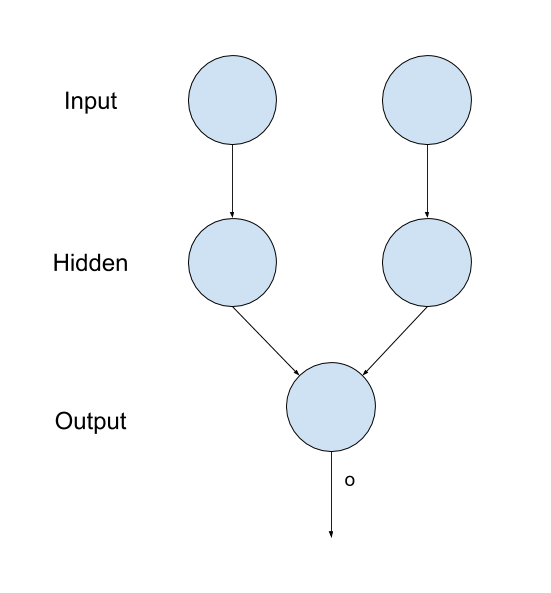
\includegraphics[width=\textwidth]{implys-nand-net.png}
    \caption{}
    \label{fig:implys-nand-net}
  \end{minipage}
  \hfill
\end{figure}

Figure \ref{fig:implys-nand-net} demonstraits the structure a feedfoward network attempting to represent implys would look like. For $o$ to be the output required then one node in the hidden layer would have to act as an identiy, passing the input $p$ to the ouput neuron. NAND cant act as an identity.